\documentclass[11pt]{article}
\pdfinfoomitdate=1
\pdftrailerid{}
\usepackage[margin=1in]{geometry}
\usepackage[T1]{fontenc}
\usepackage{lmodern}
\usepackage{microtype}
\usepackage{amsmath,amssymb}
\usepackage{booktabs}
\usepackage{float}
\usepackage{xcolor}
\usepackage{tikz}
\usetikzlibrary{arrows.meta,positioning}
\usepackage{hyperref}
\hypersetup{
  colorlinks=true,
  linkcolor=blue,
  citecolor=blue,
  urlcolor=blue,
  pdftitle={ACSD: Authorized Lineage for Anonymous Scholarly Releases},
  pdfauthor={}
}
\newcommand{\workid}{\textsf{WorkID}}
\newcommand{\releaseid}{\textsf{ReleaseID}}
\newcommand{\acsd}{\textsc{ACSD}}
\newcommand{\sha}{\textsf{SHA-256}}
\title{\acsd: Authorized Lineage for Anonymous Scholarly Releases}
\author{Anonymous authors}
\date{}

\begin{document}
\maketitle

\begin{abstract}
Anonymous scholarly disclosure needs a more precise answer than ``put a signed PDF in a repository.'' A signature identifies a signing key, not necessarily a person; a repository timestamp is not independent time; and an exact predecessor hash does not say who may publish the next version. This paper presents \acsd, a narrow executable profile for anonymous scholarly releases and authorized lineage. A compact approval target binds exact release, governance, provenance-policy, and lineage-transition digests before every required pseudonymous key signs it. An unchanged predecessor authority can authorize an exact child through those same approvals; a key-set or threshold change additionally requires a predecessor-quorum set of signatures over the exact transition. The optional series layer remains separate, permitting cyclic semantic citation while exact release commitments stay acyclic. The implementation uses tagged Ed25519/EdDSA COSE, a closed capability calculus, and independently pinned RFC~3161 evidence. Evaluation includes an executable fresh-key n+1 attack, authorized rotation and fork cases, 64 fixed and 1,000 generated Python--Node canonical-JSON cases, adversarial timestamp tests, and 21 axiom-free Lean theorems. None of these mechanisms proves natural-person identity, contribution truth, originality, peer review, or legal nonrepudiation.
\end{abstract}

\section{Introduction}

Researchers often want to disclose a manuscript before conventional publication while keeping the author identity unavailable during review. A common informal proposal is to upload an anonymous file, sign it, and rely on repository history. That proposal leaves several distinct questions entangled.

One concrete trigger is the interval around an arXiv submission: a first-time or
new-category submission may require endorsement, while moderation and review
are separate from scientific peer review. During that interval an author may
want a public, content-anonymous evidence package that preserves exact bytes
and team assent without pretending to replace arXiv's process. We use this as
an application scenario, not as a claim that arXiv queues have a measured
backlog or that ACSD should circumvent its rules.

\begin{enumerate}
  \item What exact bytes did one or more keys approve?
  \item Can a later verifier distinguish a revision, a legitimate branch, and an equivocation?
  \item Can a sequence of papers cite one another, including mutual citations, without a circular content-hash dependency?
  \item What does a time witness establish, and what does it not establish?
\end{enumerate}

\begin{figure}[t]
\centering
\begin{minipage}[t]{0.39\linewidth}
\centering
\vspace{0pt}
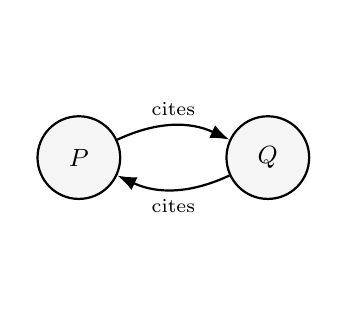
\begin{tikzpicture}[
  work/.style={draw, circle, fill=gray!8, minimum size=1.05cm,
               thick, font=\small},
  semedge/.style={-{Latex[length=2.4mm]}, thick}
]
  \path[use as bounding box] (-0.65,-1.65) rectangle (3.05,1.65);
  \node[work] (P) at (0,0) {$P$};
  \node[work] (Q) at (2.4,0) {$Q$};
  \draw[semedge] (P) to[bend left=25]
    node[above, font=\scriptsize] {cites} (Q);
  \draw[semedge] (Q) to[bend left=25]
    node[below, font=\scriptsize] {cites} (P);
\end{tikzpicture}
\par\vspace{0.24cm}\smallskip
{\small (a) Semantic graph: cycles allowed}\par
\end{minipage}
\hfill
\begin{minipage}[t]{0.57\linewidth}
\centering
\vspace{0pt}
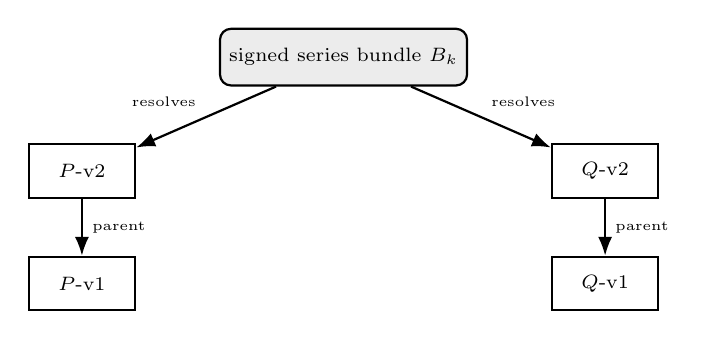
\begin{tikzpicture}[
  node distance=0.72cm and 1.05cm,
  bundle/.style={draw, rounded corners, fill=gray!15,
                 minimum height=0.72cm, minimum width=2.0cm,
                 thick, font=\scriptsize},
  release/.style={draw, rectangle, fill=white,
                  minimum height=0.68cm, minimum width=1.35cm,
                  thick, font=\scriptsize},
  dep/.style={-{Latex[length=2.4mm]}, thick}
]
  \node[bundle] (B) {signed series bundle $B_k$};
  \node[release] (P2) [below left=of B] {$P$-v2};
  \node[release] (Q2) [below right=of B] {$Q$-v2};
  \node[release] (P1) [below=of P2] {$P$-v1};
  \node[release] (Q1) [below=of Q2] {$Q$-v1};

  \draw[dep] (B) -- node[above left, font=\tiny] {resolves} (P2);
  \draw[dep] (B) -- node[above right, font=\tiny] {resolves} (Q2);
  \draw[dep] (P2) -- node[right, font=\tiny] {parent} (P1);
  \draw[dep] (Q2) -- node[right, font=\tiny] {parent} (Q1);
\end{tikzpicture}
\par\smallskip
{\small (b) Commitment graph: a DAG}\par
\end{minipage}

\caption{ACSD separates cyclic semantic citations over stable WorkIDs (a) from
acyclic exact-byte commitments through release digests and predecessor links
(b). Commitment arrows point toward the committed object and indicate neither
chronology nor priority.}
\label{fig:two-graphs}
\end{figure}

The first question is about key control and integrity. It is not, by itself, a proof that a particular natural person wrote the work. The second and third are data-model and verification questions. The fourth requires an external witness such as an RFC~3161 timestamp authority (TSA), not a local clock or a mutable Git field. Conflating these layers produces systems that overclaim.

This paper presents \acsd\ (Anonymous Scholarly Claim and Disclosure), a deliberately narrow application profile. It uses standard content hashing, COSE signatures, and provenance concepts rather than proposing a new primitive. The profile is designed for content-anonymous release: the public paper and artifact do not name authors, but an account hosting them can still be linkable. It is therefore \emph{not} described as author-unlinkable double blind publication.

The main contributions are:

\begin{enumerate}
  \item a self-contained paper-release object with ordered anonymous author slots and per-author endorsements;
  \item a two-layer construction that permits cyclic scholarly citations over stable \workid s while keeping content commitments acyclic;
  \item signed UTF-8 byte-range citation witnesses and a restricted canonical JSON profile to reduce field-interpretation ambiguity;
  \item explicit classifications for branches, equivocation, and copied content under a fresh lineage;
  \item an acyclic unanimous-approval target and closed capability calculus that prevent unsigned policy amplification and approval reuse after governance or PEC substitution;
  \item an exact lineage transition requiring predecessor-quorum signatures, rejecting a fresh-key n+1 claimant while supporting explicit author/key changes and branches; and
  \item an executable prototype with one-command release and revision paths, independent COSE verification, adversarial RFC~3161 checks, generated differential testing, and an axiom-free Lean model of the composition rules.
\end{enumerate}

\section{Scope and Threat Model}

\paragraph{Assets.} A release contains manuscript bytes, an ordered list of anonymous author keys, roles and contribution declarations, an AI-use declaration, and optional parent-release information. A series package contains references to completed releases, a series key, sequencing information, and cross-paper semantic relations. Public keys are pseudonymous identifiers.

\paragraph{Adversary.} We consider a party that can copy public content, generate fresh keys, reuse the exact WorkID and predecessor digests, claim the next unused version number, reorder or substitute unsigned metadata, present a signed but malformed JSON payload, and claim unsupported cross-paper citations. We also consider a series key that signs two incompatible objects. We do not assume that a signature reveals a human identity, that a contribution declaration is factually true, or that a local timestamp is trusted.

\paragraph{Non-goals.} \acsd\ does not prove authorship by a natural person, independent discovery, plagiarism, venue acceptance, peer review, or legal nonrepudiation. These are not merely unimplemented features: some require social, institutional, or legal evidence outside the cryptographic object. The profile instead preserves evidence that can be useful in a later dispute.

\section{Release Layer}

\subsection{Canonical release object}

Each \emph{PaperRelease} has a random stable \workid, a visible slot $(\workid,\textit{version},\textit{line})$, a content path, content length and digest, ordered author records, declared roles, contributions, an AI-use declaration, optional exact predecessor, and a list of citation witnesses. The release identifier is
\[
  \releaseid = \texttt{urn:sha256:}H(\mathrm{canonical}(R)).
\]
The content digest is over exact manuscript bytes. The release object uses a deliberately restricted JSON encoding: recursively sorted ASCII object keys, no insignificant whitespace, and safe integers only. A verifier parses, re-canonicalizes, and compares bytes before accepting a signature. This is a profile rule, not a claim that it is a general JSON standard.

\subsection{Joint approval target and closed capability calculus}

The \emph{AuthorshipGovernanceStatement} is the exact declaration of the work
id, manuscript digest, ordered byline slots and roles, corresponding-author key,
and AI-use field. The CLI derives it from the team configuration and release;
there is no privileged coordinator whose unsigned word makes it authoritative.
Instead, every declared author key approves its digest through the common
target described below. This proves assent to the declaration, not the factual
truth of its roles or contribution history.

A \emph{Provenance Evidence Capsule} (PEC) binds the release subject and
governance digest to a digest-linked evidence-event sequence and a claim
policy. The policy contains a fixed-vocabulary list of permitted outcomes,
their required capabilities, and mandatory non-claims. A PEC also names one
team key as an issuer for provenance, but that label alone grants no outcome:
the complete team must still approve the common target.

The v3 command-line profile constructs an acyclic
\texttt{acsd-approval-target/v2} object. It points to already complete objects
and is itself signed only through detached approval envelopes. The following is
a structurally valid, pretty-printed example with illustrative digest values:

\begingroup\scriptsize
\begin{verbatim}
{
 "schema":"acsd-approval-target/v2",
 "work_id":"urn:uuid:12345678-1234-1234-1234-123456789abc",
 "release_digest":"1111111111111111111111111111111111111111111111111111111111111111",
 "governance_digest":"2222222222222222222222222222222222222222222222222222222222222222",
 "pec_digest":"3333333333333333333333333333333333333333333333333333333333333333",
 "required_key_ids":["4444444444444444444444444444444444444444444444444444444444444444"],
 "lineage_transition_digest":null
}
\end{verbatim}
\endgroup

Every required key issues a tagged COSE Sign1 signature over the same
canonical target bytes. Verification recomputes all four bindings and each key
id from the supplied public key. The closed capability calculus is the rule
\[
 \mathrm{Granted}(P,o) \iff \mathrm{Accepted}(P)
 \land o\in P.\mathrm{permittedOutcomes}
 \land \mathrm{CapabilityEstablished}(P,o).
\]
Policy permission is therefore only an upper bound; it is not evidence. The
outcome type is closed to four machine conclusions, so an unknown social claim
cannot enter the rule by adding a string to JSON.

Without the joint target, suppose authors sign only the release while an
attacker later changes the unsigned governance object or PEC policy. The
attacker could relabel roles, add the external-time outcome, or try to map a
local clock to that outcome while the old release signatures still verify.
Under ACSD, changing the governance or policy changes its digest and causes a
target-binding failure; recomputing the target instead causes the old COSE
approvals to fail their payload check. Even an approved policy entry yields no
outcome without its separately verified capability. A verifier can thus state
that the pseudonymous keys jointly approved this exact tuple, but cannot infer
who controls them without separate enrollment evidence.

\subsection{Authorized succession rather than version-number possession}

An exact predecessor digest proves structural continuity, not authority. A
fresh-key attacker can copy a public WorkID, name the real predecessor, choose
the consecutive version number, and validly sign the resulting child with the
attacker's keys. No hash or slot-conflict check answers whether those keys were
entitled to create the parent-to-child edge. ACSD v3 therefore binds every
release to a \emph{lineage authority}: a sorted author-key set and a threshold
for authorizing the next edge. The default threshold is unanimity. It is stored
in the predecessor, so a child cannot lower it unilaterally.

Let $P$ be an accepted predecessor, $C$ a proposed child, $A_P$ the authority
bound by $P$, and $A_C$ the authority proposed by $C$. The verifier accepts a
lineage edge only if
\[
 \mathrm{AuthorizedSuccessor}(P,C) = \mathrm{ExactEdge}(P,C) \land
 \mathrm{Authorization}(P,C),
\]
where
\[
 \mathrm{Authorization}(P,C)=
 \begin{cases}
  \mathrm{Quorum}(A_P,\mathrm{ApproveTarget}(C)), & A_P=A_C,\\
  \mathrm{Quorum}(A_P,\mathrm{Transition}(P,C)) \land
  \mathrm{AllApprove}(A_C,C), & A_P\ne A_C.
 \end{cases}
\]
Here \textsf{ExactEdge} requires the same WorkID, exact parent release and PEC
digests, and either a same-line increment by one or a new named line beginning
at version one. \textsf{Transition} binds both authorities and the exact child
release, governance, and PEC digests. The child approval target binds the
transition digest. The construction is acyclic because the transition refers
to complete child bodies while detached approvals refer to their completed
digests.

For an unchanged authority object, the ordinary child approvals already constitute
predecessor authorization and no duplicate signing step is needed. A key-set or
threshold change uses double control: the predecessor threshold signs the exact
transition and every new author signs the child target. This resembles the
old-and-new authorization pattern used for TUF root-key updates, but ACSD
applies it to a single scholarly lineage edge rather than software repository
metadata~\cite{tufspec}. A series key may advertise a verified child as a head;
it cannot manufacture predecessor-author assent by itself.

Consider the concrete n+1 attack. Mallory constructs a child with P's WorkID,
P's exact release and PEC digests, the next version number, Mallory's public
key, and a valid Mallory signature over every child-controlled object. The
object is internally signed but has neither an unchanged predecessor authority
nor a transition signed by $A_P$. The implementation returns
\texttt{VALID\_OBJECT\_BUT\_UNAUTHORIZED\_SUCCESSOR}. It does not accuse
Mallory of plagiarism; it rejects only the claimed lineage edge.

This conclusion is relative to an accepted exact predecessor, not to the
WorkID string alone. The CLI can pin a previously accepted parent with
\texttt{--expected-parent-release-id}; otherwise it reports
\texttt{UNPINNED\_EXACT\_PARENT}. Without an external parent anchor, an isolated
package proves only that the authority named by its embedded parent authorized
the edge; it cannot distinguish a separately fabricated genesis that copied a
public WorkID.

Threshold choice exposes a real safety--liveness tradeoff. Unanimity prevents
one coauthor from transferring the lineage alone but lets one lost or dissenting
key freeze it. A lower threshold improves availability and is therefore allowed
only when committed by the predecessor. There is no post-hoc identity recovery
in this profile: without a precommitted recovery authority, lost threshold keys
safely stop the cryptographic lineage. Nor can a later message erase a valid
past authorization. Two valid distinct children in the same exclusive slot are
reported as equivocation with no automatic winner; choosing by observation time
requires an external transparency or governance policy.

\subsection{Citation witnesses}

The prototype recognizes only literal occurrences of a canonical token \texttt{urn:uuid:<work-id>} in the UTF-8 manuscript bytes. For every occurrence it records and signs
\[
  (\workid,\ \textit{byteOffset},\ \textit{byteLength}).
\]
The published \texttt{reference\_work\_ids} list must equal the ordered de-duplicated projection of these witnesses. This prevents a series package from inventing a citation edge that has no corresponding token in its source release, and prevents a copied text from silently relabeling an old target as a new \workid.

The rule intentionally does not parse PDFs, infer references from natural language, or determine whether a citation is intellectually appropriate. It is an exact byte-binding contract, not a semantic understanding claim.

For example, one UTF-8 source line contains the following token:
\begin{verbatim}
urn:uuid:12345678-1234-1234-1234-123456789abc
\end{verbatim}
The witness records that WorkID, the byte offset of the first character of the
token, and its byte length (45 bytes for this token). An editor that inserts a
character before the token must regenerate the witness. This is intentionally
mechanical: a source-level helper or build macro can insert the token, but v1
does not yet provide such editor integration, and hiding the token in a PDF
would defeat this scanner.

A minimal release fragment is conceptually:
\begin{verbatim}
{"slot":{"line":"main","version":1,"work_id":"urn:uuid:..."},
 "content":{"sha256":"..."},
 "reference_work_ids":["urn:uuid:..."],
 "citation_witnesses":[{"work_id":"urn:uuid:...",
   "byte_offset":35,"byte_length":45}]}
\end{verbatim}
The ellipses above are presentation placeholders only. The released demo
fixture binds a real manuscript's bytes, digest, and work identifier (the
governance and PEC objects are real, not placeholders), using synthetic author
identifiers. Real series releases are produced by the v1 fixture generator.

\section{Series Layer and Cyclic Citations}

\subsection{Two graphs, two purposes}

A paper remains verifiable after all series packages are removed. The optional series layer records relationships among independently complete releases. A signed series package contains
\[
\begin{aligned}
  B_k = \mathrm{Sign}_{S}(&\textit{seriesId},\textit{epoch},\textit{sequence},\textit{previousBundleHash},\\
                           &\textit{rotationHash},\textit{rank},\textit{releases},\textit{heads},\textit{semanticEdges}).
\end{aligned}
\]

The semantic graph has vertices \workid s and may contain $P \rightarrow Q$ and $Q \rightarrow P$. Its edges express declared citation or related-work relations. The commitment graph has series anchors and completed \releaseid s. It does not make a release depend on a future series package. Thus two authors can cite stable random \workid s before both final documents are content-addressed; a later package resolves each \workid to a completed \releaseid. The semantic graph may be cyclic while the commitment graph remains a DAG.

The package includes a signed structural rank strictly above every release version it resolves. Combining anchor-to-release edges with exact release-to-parent edges decreases this rank along a commitment path. This rank is a graph certificate, not a timestamp, publication date, or priority claim.

The package fields have narrow roles: \textit{epoch} names the active series
key generation; \textit{rotationHash} commits its authorized key transition;
\textit{heads} maps each WorkID to its advertised line head; and
\textit{semanticEdges} records declared citation or related-work relations.
The rank is only a finite measure certifying that the commitment graph has no
cycle.

\subsection{Revisions, branches, and conflicts}

A revision names one exact predecessor. Multiple children of a parent are allowed, because a main manuscript and a computational appendix can be legitimate independent lines. A paper-level equivocation is instead detected when two valid, different releases occupy the same exclusive slot. A series-level equivocation is detected when two valid packages share the same series, epoch, sequence, and predecessor hash while committing to different contents.

An adversary can copy the content bytes, issue a fresh \workid and keys, and obtain a valid new lineage. \acsd\ classifies this as content reuse under a different lineage, not as a cryptographic proof of plagiarism. That restraint is important: reuse may be authorized, collaborative, or independently derived.

As a concrete attack, suppose an attacker copies P-v1, changes its WorkID,
and asks the series package to claim that it cites Q. The release verifier
recomputes the content digest and byte witnesses; if the copied source does not
contain the declared Q token, the package is rejected as an unsupported edge.
If the attacker copies the token too, the package can still be valid under a
new lineage. The evidence then says only “content reuse under a different
lineage”; deciding plagiarism or authorization remains outside the verifier.

\section{Time Evidence}

Time is intentionally external to author signing. An RFC~3161 request contains
the \sha\ imprint of the frozen approval target. A response supports the limited
statement that the TSA saw that imprint no later than its recorded
\texttt{genTime} only when the verifier supplies a TSA signer-certificate or
fingerprint pin independently of the package. A certificate and its fingerprint
copied into the same mutable package are not a trust anchor. The adapter checks
the request/response nonce, SHA-256 imprint, \texttt{id-ct-TSTInfo} content type,
single signer identifier, critical and exclusive timeStamping EKU, ESS
certificate identifier, signed attributes, and CMS signature. It implements an
exact-signer pin, not general PKIX path construction or revocation. Its local
test TSA is a protocol test and can never produce
\texttt{EXTERNALLY\_NOT\_AFTER}.

There is no circularity: the timestamp receipt is a sidecar over the already
signed target. A later revision can bind the receipt hash if a new signed object
must refer to it. A timestamp does not prove creation at that moment,
authorship, originality, or global first discovery. Multiple independently
governed services can reduce single-service reliance, but their composition
requires a separate policy.

\section{Implementation and Evaluation}

The v1 prototype uses Python for deterministic fixture generation and a zero-dependency Node.js verifier for strict CBOR/COSE and profile validation; the two paths are intentionally separate. The package is designed for offline replay: locked dependencies are included, and the verification driver regenerates fixtures, verifies a standalone release, independently verifies the series profile, builds a manifest, and verifies that manifest.

A command-line tool (\texttt{acsd.py}) turns the profile into an executable workflow: \texttt{keygen}, \texttt{init}, \texttt{authorize}, \texttt{approve}, \texttt{finalize}, \texttt{verify}, and \texttt{compare-successors}, plus one-command \texttt{release} and \texttt{revise} paths. Approval status is derived from verified COSE files, never trusted from mutable state metadata. COSE uses the registered EdDSA value $-8$, requires tag 18, and rejects non-minimal or ambiguous CBOR encodings. A zero-dependency Node path independently verifies Python-produced approvals. The canonical JSON layer is exercised by 64 fixed Python--Node vectors plus 1,000 seeded generated cases; all generated cases agree on canonical bytes and text-layer verdicts. Three known object-layer float typing differences do not change the text-layer rejection result and remain recorded in the canonical specification.

The negative corpus includes the inherited rank, unsupported-edge,
citation-offset, canonical-JSON, and path attacks. New cross-layer regressions
replace a public key under an old key id; coherently replace governance and PEC;
recompute an unsigned target and attempt to reuse old approvals; alter COSE tags,
algorithm identifiers, map keys, and lengths; replace a timestamp and rewrite
the transport manifest; mismatch the nonce, signer, EKU, TSTInfo content type,
or signature algorithm; and attempt to promote the local test TSA. All are
rejected at their intended boundary. The single freeTSA result is an existence
check that the adapter can consume one real service response, not a reliability
study or a multi-provider conformance survey.

The lineage corpus begins with the smallest discriminating attack: a child
with the exact WorkID and parent release/PEC digests, n+1, a fresh attacker
key, and complete self-approval. It is rejected at the missing
predecessor-quorum boundary. Positive cases cover unchanged authority, key
rotation, one-of-two and two-of-two thresholds, and a named branch; negative
cases cover threshold downgrade and transition-signature replay. Two valid
same-slot siblings yield equivocation with no winner.

\begin{table}[H]
\centering
\caption{Executable evaluation corpus. The first seven rows are inherited v1 fixture results; the remaining rows are reproducible from v3.}
\begin{tabular}{lr}
\toprule
Object or check & Count / result \\
\midrule
Standalone release versions & 8 / 8 valid without series packages \\
Author endorsements & 18 / 18 bound to the intended release \\
Signed series objects & 7 \\
Closed normal, attack, and indeterminate scenarios & 13 / 13 expected outcomes \\
Independent profile checks & 30 / 30 passed \\
Canonical JSON regression cases & 11 / 11 Python--Node agreement \\
Public-manifest entries & 113 / 113 verified \\
v3 differential canonical-JSON vectors & 64 / 64 accept/reject agreement \\
Offline v3 unit-test methods & 59 passed; 1 network test skipped \\
Seeded generated canonical cases & 1000 / 1000 byte and verdict agreement \\
Independent approval implementations & Python producer / Node verifier \\
Authorized-lineage scenarios & 8 / 8 expected outcomes \\
Real-TSA existence check & 1 freeTSA response verified \\
PEC and lineage theorems in the abstract core & 21; no \texttt{sorry}/\texttt{admit} \\
\bottomrule
\end{tabular}
\end{table}

The measurements remain prototype-scale rather than a throughput claim. They
were recorded under Python 3.12.14 on 64-bit Windows 10.0.26200, a 13th Gen
Intel Core i7-1360P with 16 logical processors, and 31.7 GiB physical memory.
In that run, five repetitions of an in-memory workload that canonicalizes
objects, constructs and verifies SHA-256 manifest entries, and scans a linear
rank certificate had median times of 2.23, 26.45, 227.54, and 718.81 ms for
10, 100, 1,000, and 5,000 objects respectively; peak traced memory at 5,000
objects was 7.04 MiB. This excludes filesystem, COSE, and network cost, so it
is a smoke test for obvious scaling anomalies, not a statistically powered
performance evaluation; dispersion beyond minimum and median was not retained.

The v3 Lean development uses concrete approval targets, approvals, digest-linked
events, a closed outcome type, decomposed time evidence, and typed lineage
authorities and transitions. Its 21 theorems
prove, among other facts, that an approval for one target digest cannot be
reused for a different target; a granted result implies acceptance and policy
permission; key assent requires all target approvals; and external time
requires exact-subject, signer-pin, nonce, profile, and non-local predicates.
The lineage theorems show that every accepted successor has predecessor-quorum
evidence, a fresh authority cannot enter through the unchanged-authority path,
and a transition bound to one child digest cannot authorize another child.
The model deliberately accepts signature validity and digest equality as inputs.
It does not prove parser refinement, SHA-256 collision resistance, Ed25519
unforgeability, TSA honesty, or general PKIX correctness.

These 21 are PEC, lineage, and cross-layer composition theorems, not a recount of the
separately published v1 Lean core.\footnote{The v1 proof surface is archived at
\url{https://github.com/huiminZheng-collab/acsd-anonymous-series-v1/tree/main/formal-core}.}
The v1 artifact records 53 theorem statements
about release catalogs, teams, lineage, series graphs, citation witnesses, and
lifecycle rules. That earlier model remains an inherited, distinct proof
surface; it was neither deleted nor compressed into the new count. The v3
count concerns the narrower executable model of approval-target reuse,
capability gating, event links, external-time preconditions, and authorized
succession.

\section{Related Work}

The profile builds on established foundations. PROV-DM supplies a general vocabulary for entities, activities, agents, derivations, and bundles~\cite{prov}. Software Heritage identifiers provide intrinsic identifiers for software objects~\cite{swhid}; Trusty URIs provide hash-bearing immutable artifact identifiers~\cite{trusty}. COSE defines the signed binary envelope used for endorsements~\cite{cose}. SCITT specifies a broader architecture for signed statements and transparency receipts~\cite{scitt}. RFC~3161 specifies the timestamp protocol~\cite{rfc3161}. TUF uses predecessor and successor root thresholds to preserve trust through root-key updates~\cite{tufspec}; in-toto binds supply-chain steps to authorized functionaries~\cite{intoto}. These are the closest authorization patterns, although neither specifies anonymous scholarly WorkID succession.

\acsd\ does not claim to replace these systems or invent threshold delegation. Its narrow contribution is an executable scholarly profile that combines: self-contained anonymous paper releases; exact predecessor-authorized succession; a separate series layer for mutual citations; exact text-token witnesses; explicit conflict predicates; and counterexamples against common overclaims about signatures, local clocks, and copied content.

\begin{table}[H]
\centering
\caption{Capability boundary (not a performance comparison).}
\begin{tabular}{p{0.23\linewidth}p{0.29\linewidth}p{0.36\linewidth}}
\toprule
System & Primary capability & ACSD boundary \\
\midrule
OpenTimestamps & Blockchain-anchored timestamp proofs & Optional time sidecar; no author-role or citation semantics \\
Software Heritage / SWHID & Persistent intrinsic identifiers for archived software objects & ACSD binds scholarly release roles, declarations and paper relations \\
Zenodo & Versioned archival record and DOI & ACSD's byte-level policy and pseudonymous team assent remain explicit \\
RFC 3161 & TSA-signed message-imprint time evidence & Exact not-after evidence only; never authorship or originality \\
TUF / in-toto & Threshold key update and authorized software-supply-chain functionaries & ACSD scopes old/new authority to exact scholarly child objects \\
ACSD & Release, governance, authorized revision, witness and claim-policy profile & Composes these boundaries while retaining backend trust assumptions \\
\bottomrule
\end{tabular}
\end{table}

\section{Limitations and Future Work}

Several extensions are intentionally deferred. First, relations across independently administered series require policy and an interoperable cross-series package model. Second, anti-equivocation evidence from transparency logs or gossip requires deployed service assumptions. Third, the parser, threshold counter, canonicalization, hash, and signature implementations have not been refined into the Lean model. Fourth, generated private keys are unencrypted PEM files; a production CLI needs encrypted or operating-system-backed storage. Fifth, exact TSA signer pinning does not replace PKIX path construction and revocation when a deployment requires those services. Sixth, v3 has no precommitted recovery authority: loss of enough predecessor keys freezes the lineage, while an already valid transfer cannot be retroactively revoked. Finally, content-anonymous publication does not hide repository-account, network, timing, or public-key linkage, and richer citation/editor integration remains future work.

These are reasons to state the present result narrowly, not reasons to weaken the useful evidence it already preserves.

\section{Conclusion}

\acsd\ turns a vague ``anonymous signed paper'' idea into a limited but executable evidence profile. It binds exact released objects to pseudonymous-key approvals, distinguishes a signed object from a predecessor-authorized successor, supports ordered roles and branches, permits mutual scholarly citation without cyclic hash dependencies, and detects same-slot authorized forks without inventing a winner. It leaves human identity, originality, recovery without prior authority, and independent time as claims requiring additional evidence. This division of claims is the central design principle: preserve what cryptography can verify, and make the remaining social questions explicit.

\begin{thebibliography}{9}
\bibitem{prov}
W3C. \emph{PROV-DM: The PROV Data Model}. W3C Recommendation, 2013. \url{https://www.w3.org/TR/prov-dm/}

\bibitem{swhid}
Software Heritage. \emph{SWHID Specification: Core Identifiers}, version 1.2. \url{https://www.swhid.org/specification/v1.2/5.Core_identifiers/}

\bibitem{trusty}
T. Kuhn and M. Dumontier. \emph{Trusty URIs: Verifiable, Immutable, and Permanent Digital Artifacts for Linked Data}. ESWC, 2014. \url{https://doi.org/10.1007/978-3-319-07443-6_27}

\bibitem{cose}
J. Schaad. \emph{CBOR Object Signing and Encryption (COSE): Structures and Process}. RFC 9052, 2022. \url{https://www.rfc-editor.org/rfc/rfc9052.html}

\bibitem{scitt}
H. Birkholz et al. \emph{An Architecture for Trustworthy and Transparent Digital Supply Chains}. RFC 9943, 2026. \url{https://www.rfc-editor.org/rfc/rfc9943.html}

\bibitem{rfc3161}
C. Adams et al. \emph{Internet X.509 Public Key Infrastructure Time-Stamp Protocol (TSP)}. RFC 3161, 2001. \url{https://www.rfc-editor.org/rfc/rfc3161.html}

\bibitem{opentimestamps}
OpenTimestamps. \emph{A timestamp proof standard for blockchain anchoring}.
Project documentation, accessed 2026-09-11. \url{https://opentimestamps.org/}

\bibitem{tufspec}
The Update Framework. \emph{The Update Framework Specification}, version 1.0.28. \url{https://theupdateframework.github.io/specification/v1.0.28/}

\bibitem{intoto}
in-toto. \emph{in-toto Specification}. \url{https://github.com/in-toto/docs/blob/master/in-toto-spec.md}
\end{thebibliography}

\end{document}
